\documentclass[11pt,letterpaper]{article}

% ============================================================
% reflector
% Reflective Development Systems for
% Recursive AI-Augmented Software Engineering
% ============================================================

% ============================================================
% Encoding and Typography
% ============================================================

\usepackage[utf8]{inputenc}
\usepackage[T1]{fontenc}

\usepackage[english]{babel}

\usepackage{lmodern}
\usepackage{microtype}

% ============================================================
% Page Layout
% ============================================================

\usepackage[
margin=1in,
includeheadfoot,
headheight=14pt
]{geometry}

\usepackage{setspace}
\onehalfspacing%

\usepackage{parskip}

% ============================================================
% Colors
% ============================================================

\usepackage[dvipsnames]{xcolor}

\definecolor{reflectorblue}{HTML}{3B82F6}
\definecolor{reflectorpurple}{HTML}{8B5CF6}
\definecolor{reflectorgray}{HTML}{6B7280}
\definecolor{reflectorborder}{HTML}{D1D5DB}
\definecolor{reflectorbg}{HTML}{F8FAFC}

% ============================================================
% Metadata Commands
% ============================================================

\newcommand{\papertitle}{
Reflector: Reflective Development Systems for Recursive AI-Augmented Software Engineering
}

\newcommand{\paperauthor}{
Alan Szmyt
}

\newcommand{\paperdate}{
\today
}

\newcommand{\paperstatus}{
Draft
}

\newcommand{\paperrepository}{
https://github.com/egohygiene/papers
}

\newcommand{\paperorcid}{
0009-0008-5291-9795
}

\newcommand{\paperorcidurl}{
https://orcid.org/\paperorcid
}

% ============================================================
% Hyperlinks and PDF Metadata
% ============================================================

\usepackage[
unicode=true,
colorlinks=true,
linkcolor=reflectorblue,
citecolor=reflectorpurple,
urlcolor=reflectorblue,
pdftitle={\papertitle},
pdfauthor={\paperauthor},
pdfsubject={AI-Augmented Software Engineering},
pdfkeywords={
AI,
recursive systems,
governance,
human-in-the-loop,
software engineering,
recursive auditing,
milestone synchronization,
contextual synchronization,
recursive drift,
reflective systems
},
pdfcreator={LaTeX},
pdfproducer={reflector publication pipeline}
]{hyperref}

\usepackage{bookmark}

% ============================================================
% Bibliography
% ============================================================

\usepackage[
backend=biber,
style=ieee,
sorting=nyt,
giveninits=true,
maxbibnames=99,
doi=true,
url=true,
isbn=false,
eprint=true
]{biblatex}

\addbibresource{references.bib}

% ============================================================
% Graphics and Figures
% ============================================================

\usepackage{graphicx}

\graphicspath{
{figures/}
{assets/}
{diagrams/}
}

\DeclareGraphicsExtensions{
.pdf,
.png,
.jpg,
.jpeg
}

\usepackage{float}
\usepackage{caption}
\usepackage{subcaption}

\captionsetup{
font=small,
labelfont=bf,
labelsep=period
}

% Accessibility note:
% Provide descriptive captions and preserve high-resolution exports.
% Future tooling may map canonical alt-text metadata into publication formats.

% ============================================================
% Tables
% ============================================================

\usepackage{booktabs}
\usepackage{array}
\usepackage{longtable}
\usepackage{tabularx}

% ============================================================
% Code Listings
% ============================================================

\usepackage{listings}

\lstdefinestyle{reflector}{
backgroundcolor=\color{reflectorbg},
basicstyle=\ttfamily\small,
breaklines=true,
frame=single,
rulecolor=\color{reflectorborder},
numbers=left,
numberstyle=\tiny\color{reflectorgray},
commentstyle=\color{reflectorgray},
keywordstyle=\color{reflectorblue},
stringstyle=\color{ForestGreen},
showstringspaces=false,
tabsize=2,
columns=fullflexible
}

\lstset{
style=reflector
}

% ============================================================
% Math and Formal Notation
% ============================================================

\usepackage{amsmath}
\usepackage{amssymb}
\usepackage{amsthm}
\usepackage{mathtools}
\usepackage{bm}

% ============================================================
% Utilities
% ============================================================

\usepackage{enumitem}
\usepackage{csquotes}
\usepackage{multirow}
\usepackage{makecell}

% ============================================================
% Intelligent References
% ============================================================

\usepackage[nameinlink,noabbrev]{cleveref}

% ============================================================
% Callouts and Boxes
% ============================================================

\usepackage[most]{tcolorbox}

\tcbset{
colback=reflectorbg,
colframe=reflectorborder,
arc=3pt,
boxrule=0.5pt
}

\newtcolorbox{reflectorcallout}{
colback=reflectorbg,
colframe=reflectorblue,
enhanced,
breakable,
left=6pt,
right=6pt,
top=6pt,
bottom=6pt
}

% ============================================================
% Header and Footer
% ============================================================

\usepackage{fancyhdr}

\pagestyle{fancy}

\fancyhf{}

\fancyhead[L]{reflector}
\fancyhead[R]{Alan Szmyt}

\fancyfoot[C]{\thepage}

\renewcommand{\headrulewidth}{0.4pt}
\renewcommand{\footrulewidth}{0pt}

% ============================================================
% Section Styling
% ============================================================

\usepackage{titlesec}

\titleformat{\section}
{\large\bfseries}
{\thesection}
{1em}
{}

\titleformat{\subsection}
{\normalsize\bfseries}
{\thesubsection}
{1em}
{}

% ============================================================
% Title Metadata
% ============================================================

\title{
\vspace{-1.25cm}
\textbf{\Huge reflector}[0.35cm]
\Large Reflective Development Systems for\
Recursive AI-Augmented Software Engineering
}

\author{
\paperauthor\
\small\href{\paperorcidurl}{ORCID: \paperorcid}\
\small\href{\paperrepository}{\paperrepository}
}

\date{\paperdate}

% ============================================================
% Document
% ============================================================

\begin{document}

% ============================================================
% Title Page
% ============================================================

\maketitle

\thispagestyle{empty}

\vspace{0.35cm}

\begin{center}
	\small Version: \paperstatus
\end{center}

\vspace{0.5cm}

\begin{abstract}
	Recursive AI-assisted software engineering systems increasingly operate through layered cycles of autonomous generation, evaluation, and refinement. As these recursive workflows scale, the cognitive burden required for humans to maintain contextual coherence grows alongside the probability of recursive drift — a progressive divergence between intended system behavior and the evolving semantic state of the system itself.

Existing software engineering methodologies were primarily designed around human-paced iteration, bounded cognitive context, and explicit synchronization boundaries. Recursive AI-assisted systems destabilize these assumptions by accelerating execution velocity, increasing recursive complexity, and continuously mutating contextual state across autonomous development cycles.

This paper introduces \textit{reflector}, a reflective development framework designed to reduce cognitive load while preserving human intentionality, governance, and architectural coherence within recursive AI-assisted workflows. \textit{reflector} introduces synchronization boundaries, reflective auditing systems, milestone-constrained recursive execution, and scoped autonomous agents as mechanisms for maintaining contextual stability across recursive development systems.

Rather than treating governance as an external control layer, \textit{reflector} frames synchronization as a contextual recompression process through which humans and AI systems periodically re-align around stabilized semantic state representations. We argue that reflective synchronization architectures will become increasingly necessary as recursive AI-assisted development systems continue scaling in autonomy, complexity, and execution speed.
\end{abstract}

\newpage

% ============================================================
% Navigation
% ============================================================

\tableofcontents

% \listoffigures

\newpage

% ============================================================
% Main Sections
% ============================================================

\section{Introduction}
\label{sec:introduction}

Lorem ipsum dolor sit amet, consectetur adipiscing elit. Integer tincidunt, sapien nec efficitur dictum, arcu orci gravida sem, vitae suscipit leo magna vitae augue. Suspendisse potenti. Pellentesque habitant morbi tristique senectus et netus et malesuada fames ac turpis egestas.

As a layout placeholder, this section references \Cref{fig:figure1} to stabilize numbering, caption flow, and cross-reference behavior during drafting.

\begin{figure}[H]
  \centering
  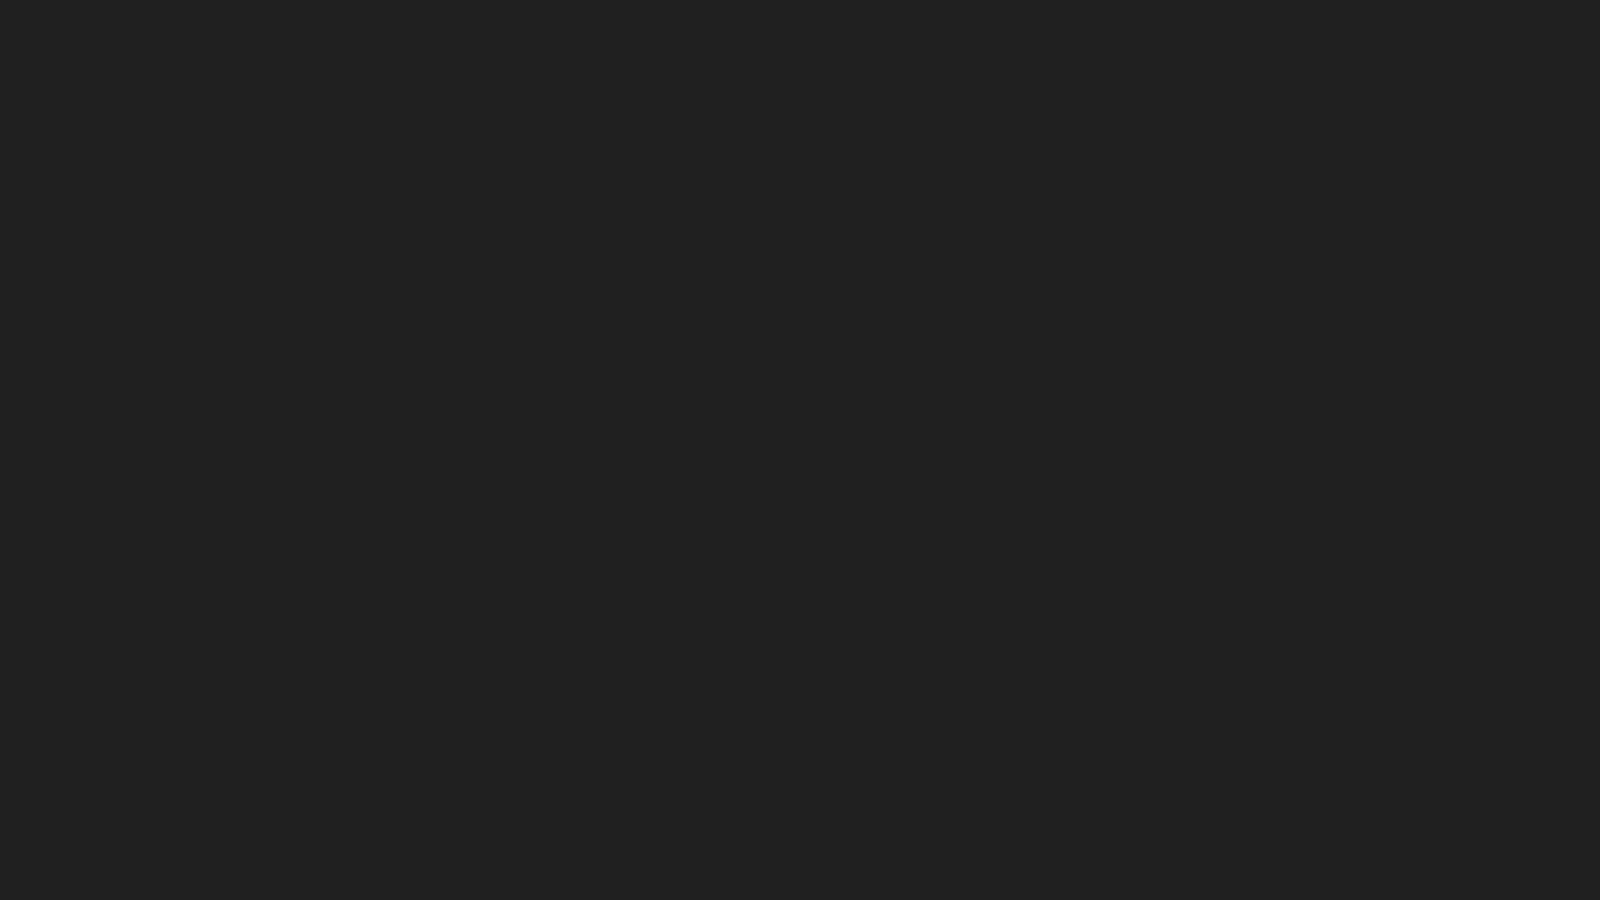
\includegraphics[width=\linewidth]{figure1.png}
  \caption{Placeholder overview figure for the introduction.}
  \label{fig:figure1}
\end{figure}

\subsection{Drafting Placeholder}

Lorem ipsum dolor sit amet, consectetur adipiscing elit. Curabitur volutpat, lorem at feugiat interdum, arcu dui pulvinar massa, vel interdum lacus augue at libero.


\section{The Emergence of Recursive AI-Assisted Systems}
\label{sec:recursive-ai-systems}

% TODO:
% Draft section on the emergence of recursive AI-assisted systems.

% Intended Figure:
% Figure 2 — Recursive AI-Assisted System Loop
% Conceptual Purpose: Illustrate layered autonomous generation/evaluation loops and human oversight touchpoints.
% Future Visual Intent: Create this visual once section arguments stabilize.


\section{Recursive Drift and Contextual Entropy}
\label{sec:recursive-drift}

% TODO:
% Draft section on recursive drift and contextual entropy.

% Intended Figure:
% Figure 3 — Drift and Entropy Progression
% Conceptual Purpose: Visualize how semantic divergence compounds over recursive iterations without synchronization.
% Future Visual Intent: Create this visual once section arguments stabilize.


\section{Synchronization, Governance, and Bounded Recursive Continuation}
\label{sec:synchronization}

If reflective auditing describes how recursive systems recover alignment, synchronization and governance define the conditions under which aligned continuation remains possible. Recursive AI-assisted systems do not merely generate outputs; they repeatedly transform those outputs into the context for subsequent execution. Each cycle therefore creates new coordination demands across artifacts, assumptions, and actors. Without explicit synchronization boundaries, recursive work can continue locally while the larger system becomes progressively less interpretable, less coherent, and less governable.

This section argues that synchronization is a stabilization requirement rather than an administrative overhead. In recursive settings, execution speed can exceed the rate at which humans can reconstruct evolving system state, and artifacts can drift out of alignment even when each local step appears reasonable. Governance layers are therefore needed to determine when autonomy may continue, when evidence must be reconciled, and when human intervention is required.

\begin{figure}[H]
  \centering
  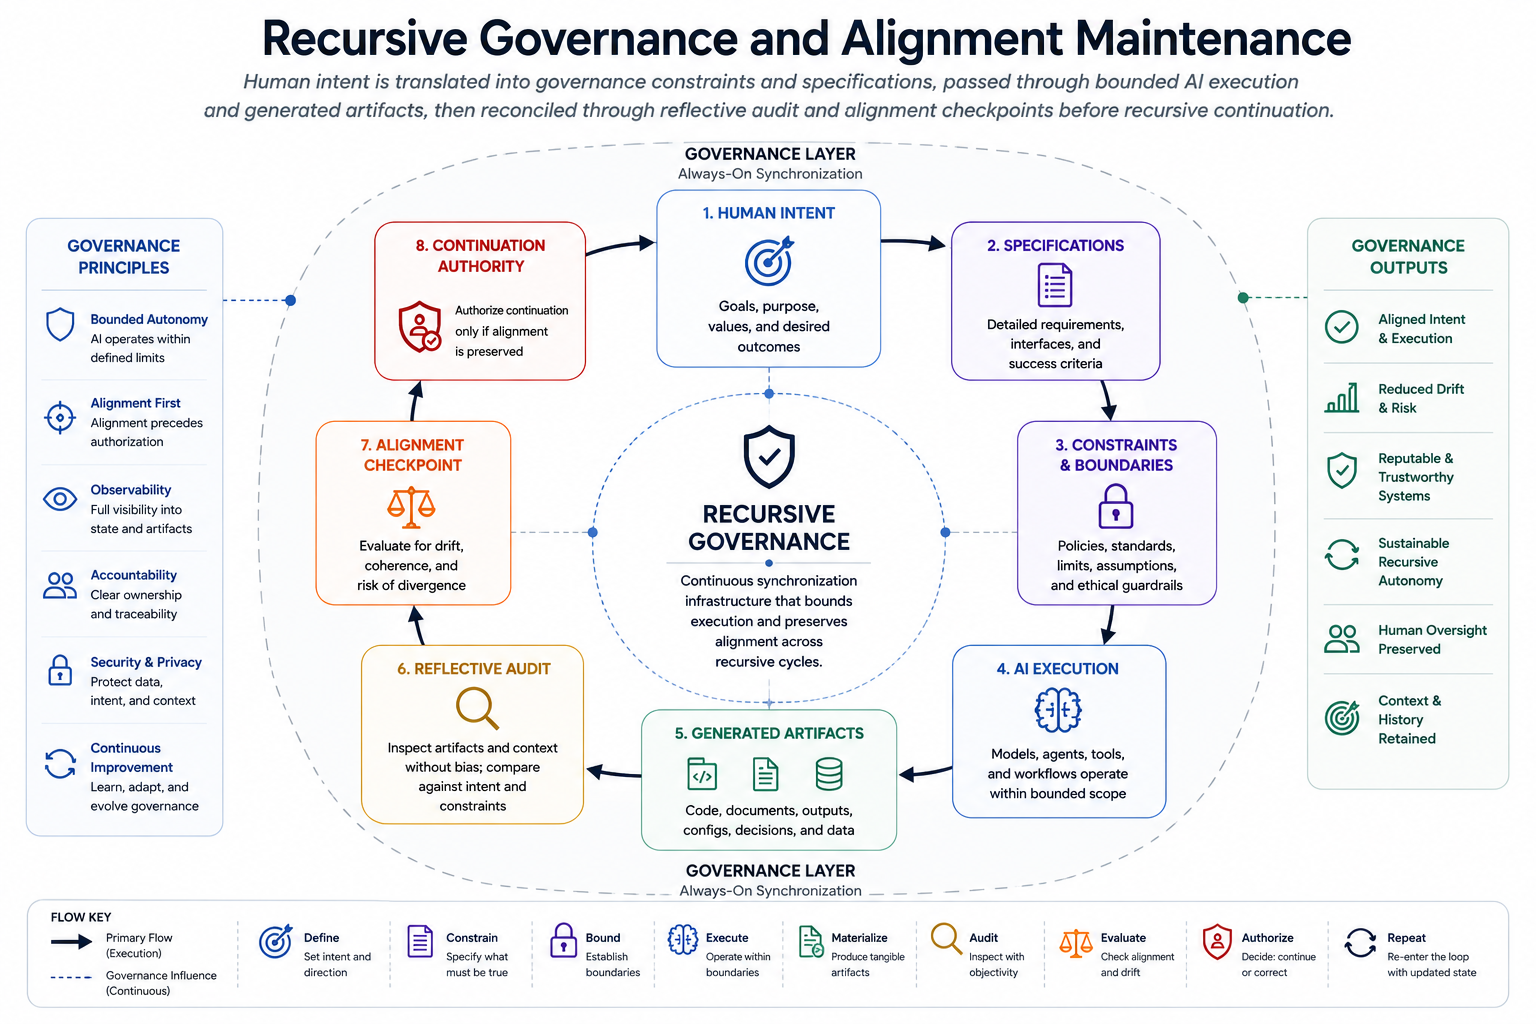
\includegraphics[width=\linewidth]{figure4.png}
  \caption{Conceptual placeholder for recursive synchronization and governance: human intent is scoped into bounded delegation, translated into AI execution and artifact generation, reconciled at synchronization checkpoints, reviewed through governance layers, and either authorized for recursive continuation or redirected for correction.}
  \label{fig:figure4}
\end{figure}

\Cref{fig:figure4} summarizes the control claim developed in this section: recursive execution remains stable only when continuation passes through explicit checkpoints that restore a shared view of scope, evidence, and authority.

\subsection{Why Recursive Systems Require Synchronization Boundaries}

Recursive systems naturally desynchronize because they operate through repeated handoffs rather than through a single uninterrupted control surface. Plans become tasks, tasks become artifacts, artifacts become summaries, and summaries become prompts for later execution. At each transformation, some meaning is compressed, omitted, or reinterpreted. The result is not necessarily immediate failure, but a gradual separation between intended scope, observed system state, and the assumptions used to justify further action.

This desynchronization pressure is intensified by asymmetric speed. AI systems can update code, tests, documentation, and workflow state faster than human operators can continuously reconstruct their combined implications. Under bounded rationality, human oversight cannot remain effective if it must infer system coherence only after multiple recursive cycles have already completed \cite{Simon1957ModelsMan,Sweller1988CognitiveLoad}. Synchronization boundaries are therefore necessary because they periodically stop local momentum long enough to produce an interpretable global snapshot.

In this sense, synchronization plays a role analogous to stabilization in distributed systems: it creates a bounded interval within which local activity may proceed, and a checkpoint at which state must be reconciled before additional propagation occurs \cite{Lamport1978TimeClocks,Chandy1985DistributedSnapshots}. For recursive AI-assisted development, the synchronized object is broader than process state alone. It includes generated artifacts, architectural assumptions, acceptance criteria, decision rationale, and the current interpretation of human intent.

\subsection{Synchronization Checkpoints as Recursive Stabilization Points}

We define a \textit{synchronization checkpoint} as an explicit boundary at which recursive execution is paused so that the current artifact set can be compared against intended scope before further delegation. Checkpoints convert a fast-moving recursive process into bounded execution intervals separated by moments of reconciliation. Their purpose is not to eliminate autonomy, but to ensure that autonomy proceeds from a refreshed and inspectable state rather than from accumulated ambiguity.

Several kinds of checkpoint are particularly important in recursive engineering workflows:
\begin{itemize}
  \item \textbf{Specification checkpoints,} where issue definitions, task decompositions, and acceptance criteria are re-synchronized before additional implementation proceeds.
  \item \textbf{Artifact checkpoints,} where code, tests, documentation, and generated plans are checked for mutual consistency.
  \item \textbf{Architectural checkpoints,} where local changes are reconciled against interfaces, invariants, and system-wide design commitments.
  \item \textbf{Milestone checkpoints,} where a bounded unit of work is evaluated for readiness to continue, integrate, or stop for revision.
\end{itemize}

These checkpoints serve as recursive stabilization points. They reduce drift by making hidden divergence observable before it becomes structural, and they create a common synchronization surface for both humans and automated systems. In practical terms, issue reviews, pull request checkpoints, architecture reviews, milestone validation, and artifact reconciliation all function as instances of the same systems primitive: bounded recursive continuation.

\subsection{Governance Layers and Bounded Autonomy}

Synchronization alone is insufficient if no authority structure determines how checkpoint evidence should affect continuation. Recursive systems therefore require \textit{governance layers}: differentiated control surfaces that decide what may be delegated, what must be reviewed, and what requires explicit approval. Governance is not introduced here as a punitive or purely bureaucratic mechanism. It is the coordination infrastructure that connects observability to authority.

At a minimum, governance operates across three layers. First, \textit{local execution governance} constrains what an AI system may do within a delegated task: files it may change, tests it must run, or specifications it must satisfy. Second, \textit{workflow governance} evaluates whether the resulting artifacts remain aligned with milestone goals, repository rules, and architectural boundaries. Third, \textit{human governance} retains final authority over scope revision, exception handling, and the decision to continue recursive execution under uncertainty \cite{Amershi2014InteractiveML,Shneiderman2020HCAI}.

This structure enables \textit{bounded autonomy}. AI systems can act with substantial local freedom, but only within scopes that preserve auditability and only until the next checkpoint requires renewed authorization. Unchecked autonomy is destabilizing not because autonomous action is inherently undesirable, but because recursive systems amplify unreviewed assumptions. A locally successful step can still deepen architectural inconsistency, encode stale requirements, or erase the rationale needed for later interpretation. Governance layers bound that amplification by ensuring that continuation remains conditional rather than automatic.

\subsection{Mixed-Initiative Stability and Human Oversight}

Recursive AI-assisted systems are mixed-initiative systems: humans and machine agents jointly participate in planning, execution, interpretation, and correction. Their strengths are complementary. AI systems accelerate search, transformation, and artifact production; humans contribute contextual judgment, normative interpretation, and the ability to resolve ambiguity that is not fully represented in the current artifact set \cite{Hutchins1995CognitionWild,Shneiderman2020HCAI}.

Human oversight in this setting should not be understood as continuous micromanagement of every local action. Such a model would collapse the throughput advantages of AI assistance without restoring recursive coherence. Instead, oversight functions as selective intervention at governance boundaries. Humans interpret whether generated evidence is sufficient, whether task scope still reflects the original objective, whether trade-offs remain acceptable, and whether the system should continue, rescope, or stop.

Mixed-initiative stability therefore depends on synchronization mechanisms that keep human interpretation coupled to machine execution. When checkpoints are absent, humans inherit only partial artifacts and delayed summaries, making it increasingly difficult to reconstruct why the system is doing what it is doing. When checkpoints are explicit, human oversight remains tractable because it engages the system at meaningful stabilization points rather than after drift has already compounded.

\subsection{Temporal Synchronization and Recursive Continuity}

Recursive systems do not only desynchronize across artifacts; they also desynchronize across time. Specifications evolve, repositories change, interfaces shift, and external constraints are updated while delegated work is still in progress. A plan that was locally valid at one checkpoint may become stale by the next. Temporal synchronization is therefore necessary to preserve continuity between past authorization and present execution.

This temporal dimension matters because recursive workflows routinely reuse prior artifacts as current context. Generated summaries, architecture notes, issue threads, and implementation diffs all become compressed representations of earlier state. If those representations are not periodically refreshed, the system continues under historical assumptions that no longer match the repository, the milestone, or the human objective. Temporal checkpoints mitigate this problem by requiring revalidation before continuation: not only ``did the system complete the task,'' but also ``is the task still the right one under the current state of the workflow?''

Synchronization thus preserves recursive continuity in two directions at once. It reconciles parallel artifacts in the present, and it reconnects current execution to the most recent valid interpretation of intent. This is what allows recursive systems to remain coherent over time rather than merely productive in isolated bursts.

Taken together, synchronization boundaries, governance layers, bounded autonomy, and human oversight define the operational conditions for stable recursive execution. Reflective auditing identifies when alignment must be examined; synchronization and governance determine how that examination structures continuation. The next section builds on these control primitives by introducing the Reflector framework as an operational recursive governance architecture that embeds checkpoints, delegation boundaries, and continuation rules directly into the development workflow (\Cref{sec:reflector-framework}).


\\section{Reflective Auditing and Perspective Cycling}
\label{sec:reflective-auditing}

Lorem ipsum dolor sit amet, consectetur adipiscing elit. Aliquam erat volutpat. Integer quis leo tempus, luctus est in, sollicitudin nulla. Sed aliquet commodo nisi, non pulvinar tortor varius at.

This placeholder subsection references \Cref{fig:figure3} to preserve stable figure sequencing in the full manuscript build.

\begin{figure}[H]
  \centering
  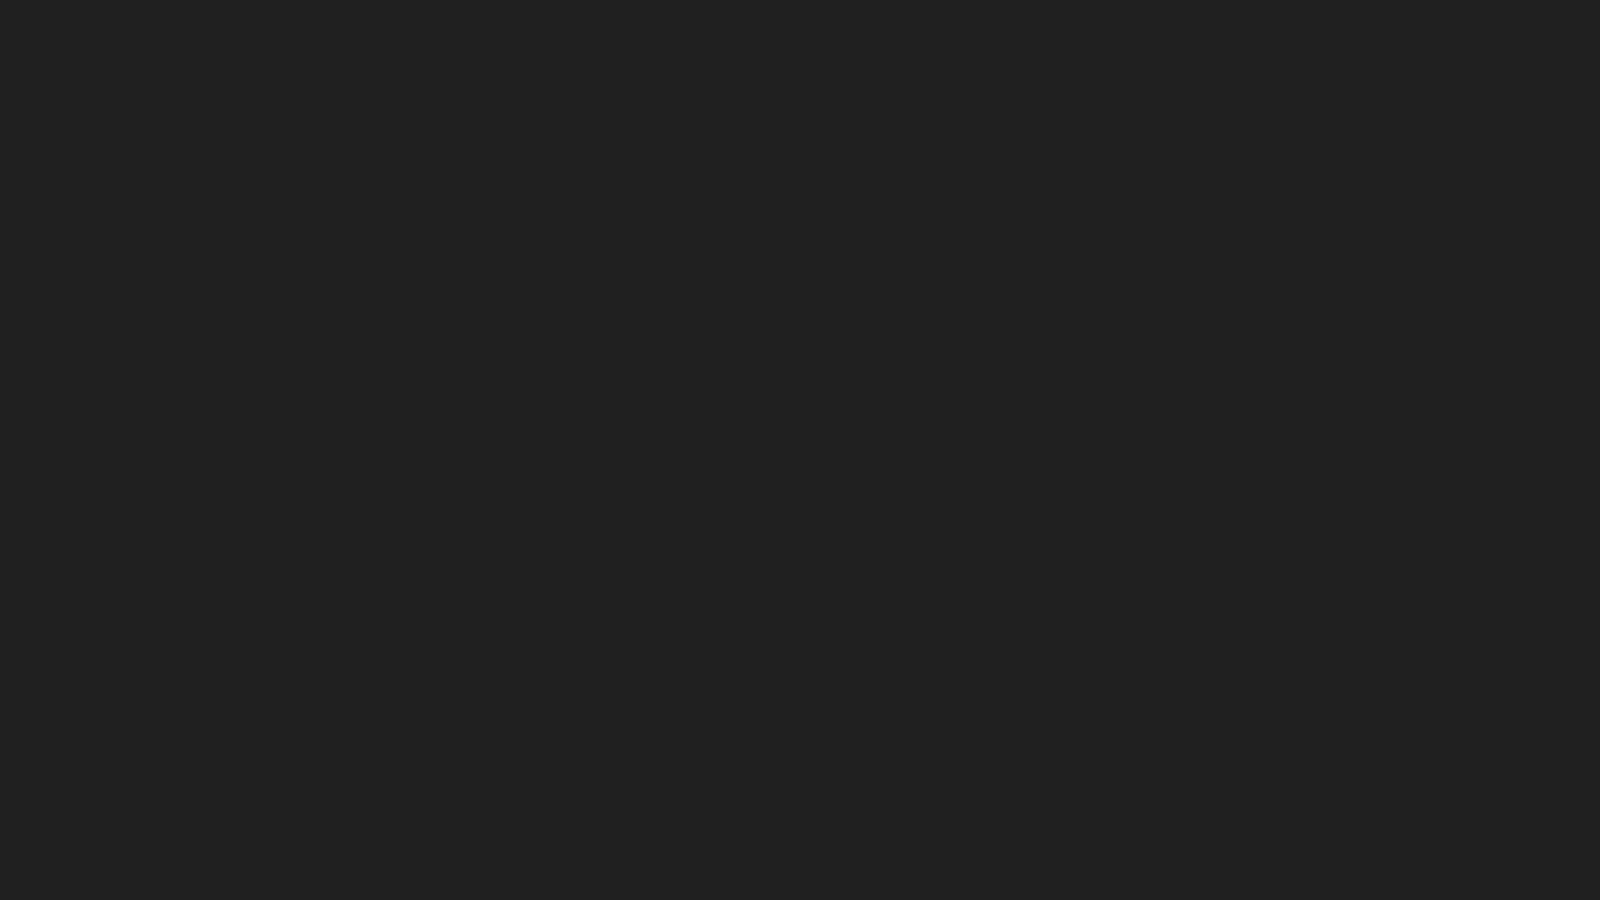
\includegraphics[width=\linewidth]{figure3.png}
  \caption{Placeholder reflective auditing cycle figure.}
  \label{fig:figure3}
\end{figure}

\subsection{Cycle Placeholder}

Lorem ipsum dolor sit amet, consectetur adipiscing elit. Integer in posuere est. Vestibulum euismod neque et nunc semper, ac ullamcorper massa viverra.


\section{Milestone-Constrained Recursive Execution}
\label{sec:milestone-execution}

% TODO:
% Draft section on milestone-constrained recursive execution.

% Intended Figure:
% Figure 6 — Milestone-Constrained Execution Timeline
% Conceptual Purpose: Map recursive execution segments to milestone gates and synchronization triggers.
% Future Visual Intent: Create this visual once section arguments stabilize.


\\section{The reflector Framework}
\label{sec:reflector-framework}

Lorem ipsum dolor sit amet, consectetur adipiscing elit. Sed efficitur justo non dolor feugiat, sed aliquet enim tristique. Integer ultricies consequat risus, sed vulputate ligula vestibulum nec.

For publication scaffolding, \Cref{fig:figure5} anchors this section's figure, caption, and reference behavior.

\begin{figure}[H]
  \centering
  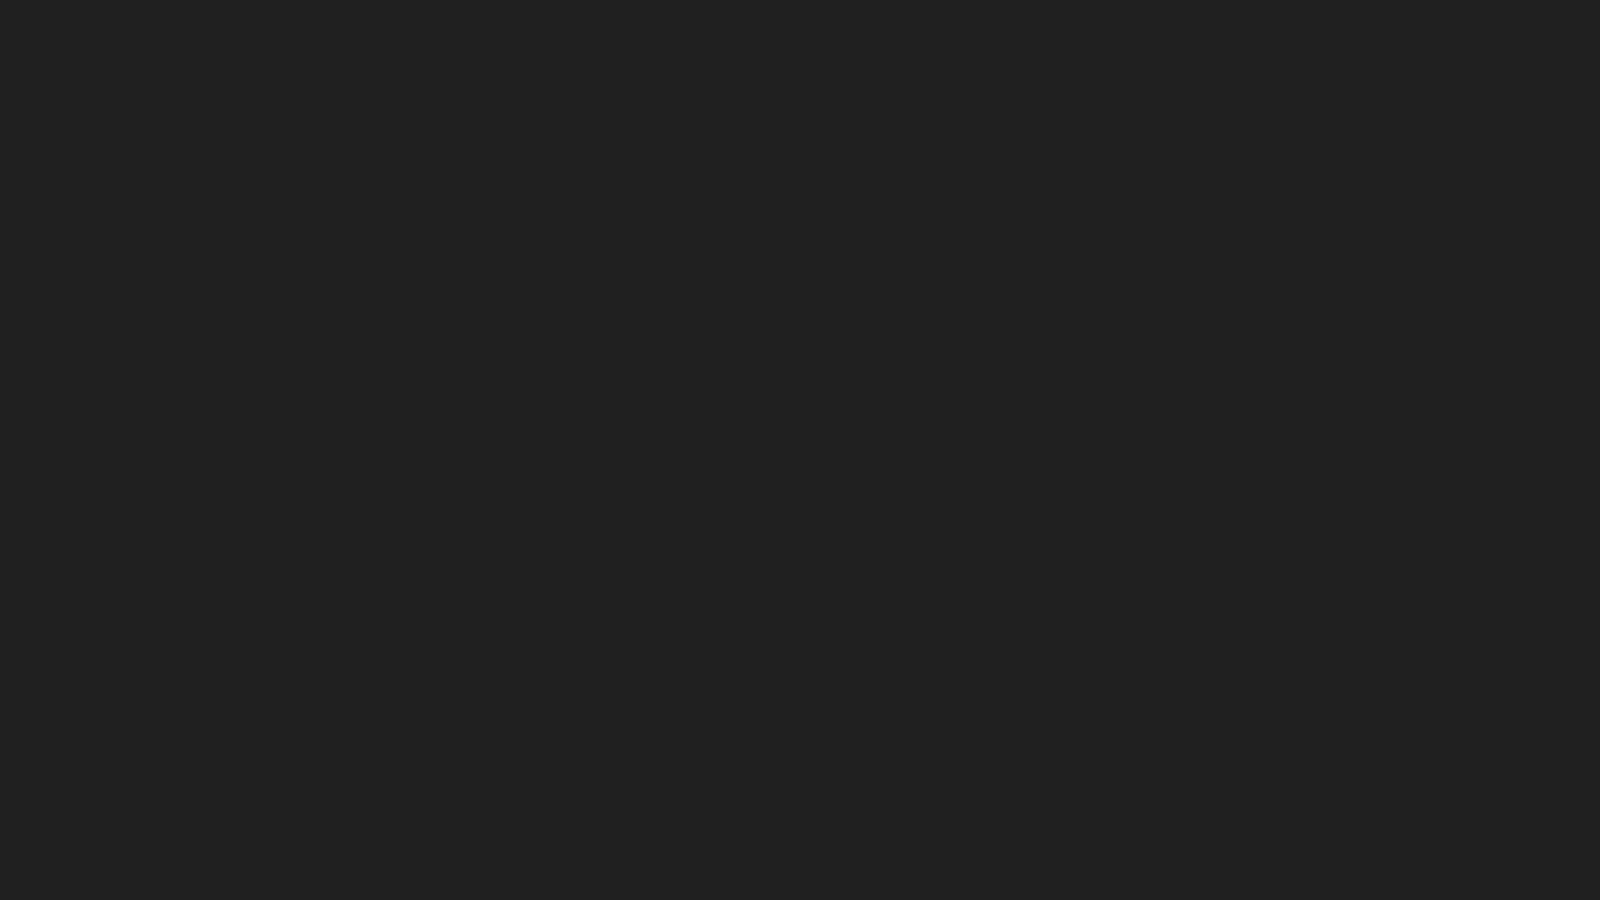
\includegraphics[width=\linewidth]{figure5.png}
  \caption{Placeholder reflector framework component map.}
  \label{fig:figure5}
\end{figure}

\subsection{Component Placeholder}

Lorem ipsum dolor sit amet, consectetur adipiscing elit. Integer eget ligula est. Mauris posuere, sem non bibendum egestas, tortor est imperdiet erat, at dignissim ligula augue at est.


\section{Operational Demonstration}
\label{sec:operational-demonstration}

Lorem ipsum dolor sit amet, consectetur adipiscing elit. Pellentesque sit amet orci ac erat ultrices tempus. Cras sit amet nunc ac justo tempus dapibus a non elit.

The current draft references \Cref{fig:figure7} to maintain deterministic figure and hyperlink structure.

\begin{figure}[H]
  \centering
  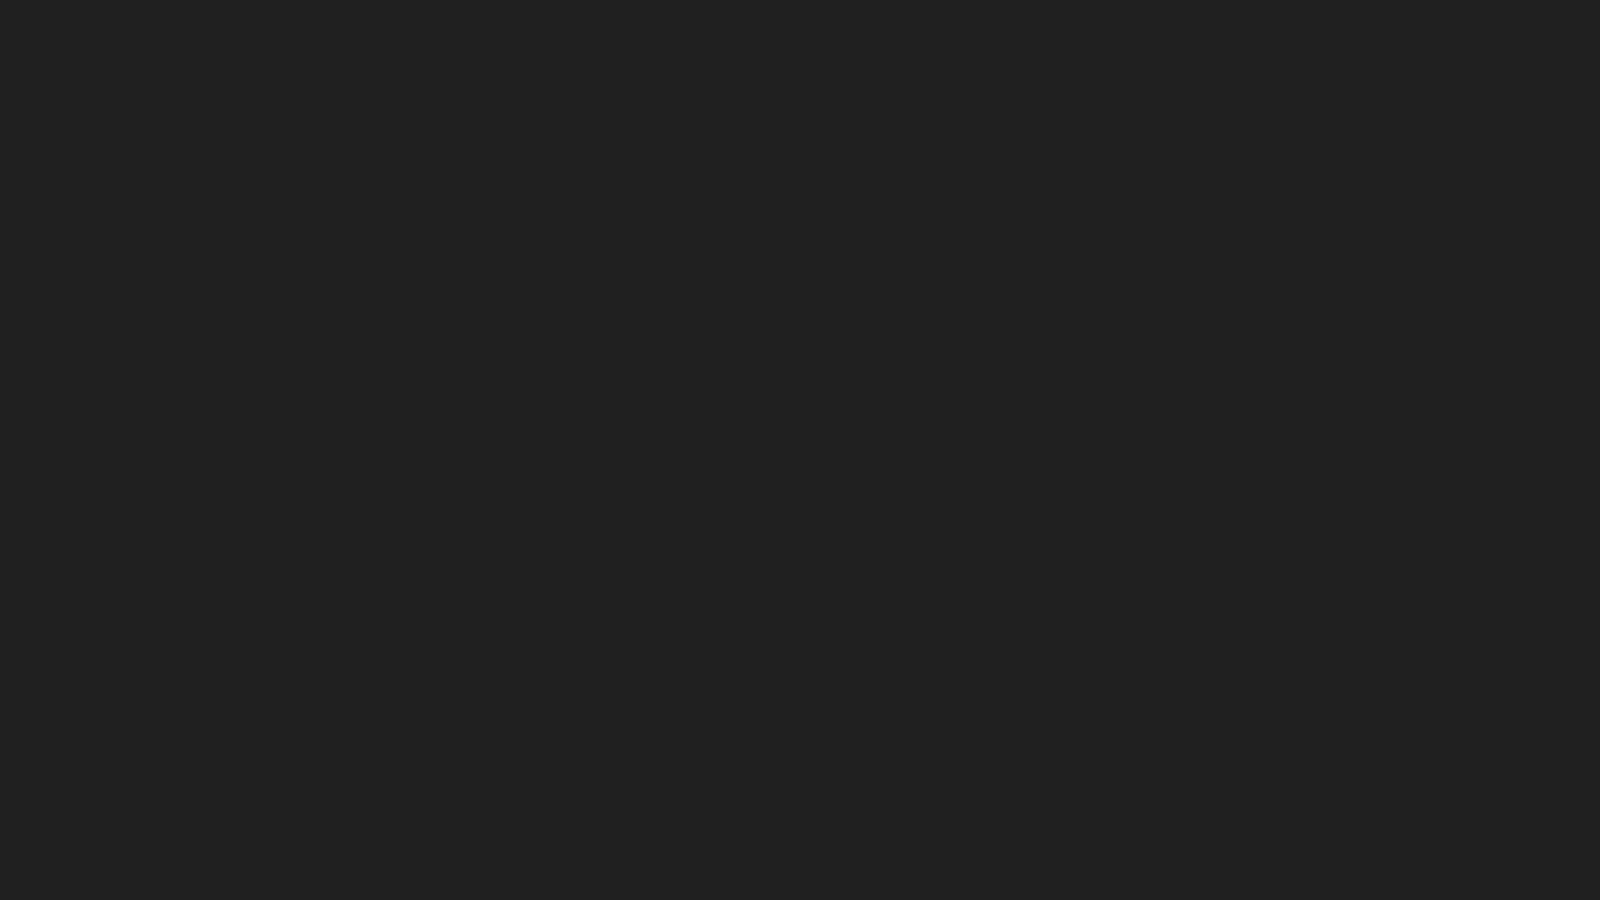
\includegraphics[width=\linewidth]{figure7.png}
  \caption{Placeholder operational demonstration flow.}
  \label{fig:figure7}
\end{figure}

\subsection{Execution Placeholder}

Lorem ipsum dolor sit amet, consectetur adipiscing elit. Donec finibus neque vel feugiat pellentesque. Sed luctus ante eget placerat feugiat.


\section{Limitations and Failure Modes}
\label{sec:limitations}

% TODO:
% Draft section on limitations and failure modes.

% Intended Figure:
% Figure 9 — Limitation and Failure Mode Taxonomy
% Conceptual Purpose: Classify known boundary conditions, failure classes, and mitigation intent.
% Future Visual Intent: Create this visual once section arguments stabilize.


\section{Conclusion}
\label{sec:conclusion}

Lorem ipsum dolor sit amet, consectetur adipiscing elit. Sed faucibus massa vel lectus consequat, vitae feugiat nisi pulvinar. In dignissim, sem vel ultrices viverra, est urna varius nunc, in suscipit purus nisl eget dui.

\subsection{Closing Placeholder}

Lorem ipsum dolor sit amet, consectetur adipiscing elit. Morbi cursus blandit ipsum, ut feugiat leo vulputate at. Integer porttitor urna sed urna pretium, at ultrices nibh congue.


% ============================================================
% Visual Summary
% ============================================================

% \section{Visual Summary}
\label{sec:visual-summary}

% TODO:
% Draft visual summary section.

% Intended Figure:
% Figure VS1 — One-Page Reflector Summary
% Conceptual Purpose: Condense the full paper into a single visual architecture and flow narrative.
% Future Visual Intent: Create this visual once section arguments stabilize.


% ============================================================
% Bibliography
% ============================================================

\newpage

\printbibliography

% ============================================================
% Appendix
% ============================================================

% \appendix
% \section{Appendix}
\label{sec:appendix}

% TODO:
% Draft appendix section.

% Intended Figure:
% Figure A1 — Supplemental Artifacts Map
% Conceptual Purpose: Reference supplementary diagrams, tables, and implementation artifacts.
% Future Visual Intent: Create this visual once section arguments stabilize.


% ============================================================
% Future Extensions
% ============================================================

% \section{Related Work}
\label{sec:related-work}

Lorem ipsum dolor sit amet, consectetur adipiscing elit. Cras a lacus felis. Nullam consequat malesuada eros, in luctus sem vulputate non. Integer posuere sem sit amet nisi commodo pulvinar.

\subsection{Positioning Placeholder}

Lorem ipsum dolor sit amet, consectetur adipiscing elit. Suspendisse non dolor at velit volutpat tempor non quis tortor. Mauris feugiat urna vel augue tempor, in ultrices lectus pretium.

% \section{Implementation Examples}
\label{sec:implementation-examples}

The operational model established in \Cref{sec:operational-demonstration} defines how recursive orchestration maintains coherence at the workflow level. The present section descends one level further---from workflow structure to implementation pattern---by demonstrating how Reflector concepts map onto concrete repository structures, specification systems, publication workflows, synchronization artifacts, and build infrastructure. The goal is not to prescribe a single production system, but to show that the architectural claims made throughout this paper are grounded in implementable, modular, and extensible engineering practices.

Each subsection below introduces a distinct implementation domain. Together they trace a path from the earliest specification artifacts through the final publication outputs, illustrating how synchronization reasoning and recursive governance can be embedded at each stage of a real engineering workflow \cite{Brooks1987NoSilverBullet,Parnas1972Modularization}.

\begin{figure}[H]
  \centering
  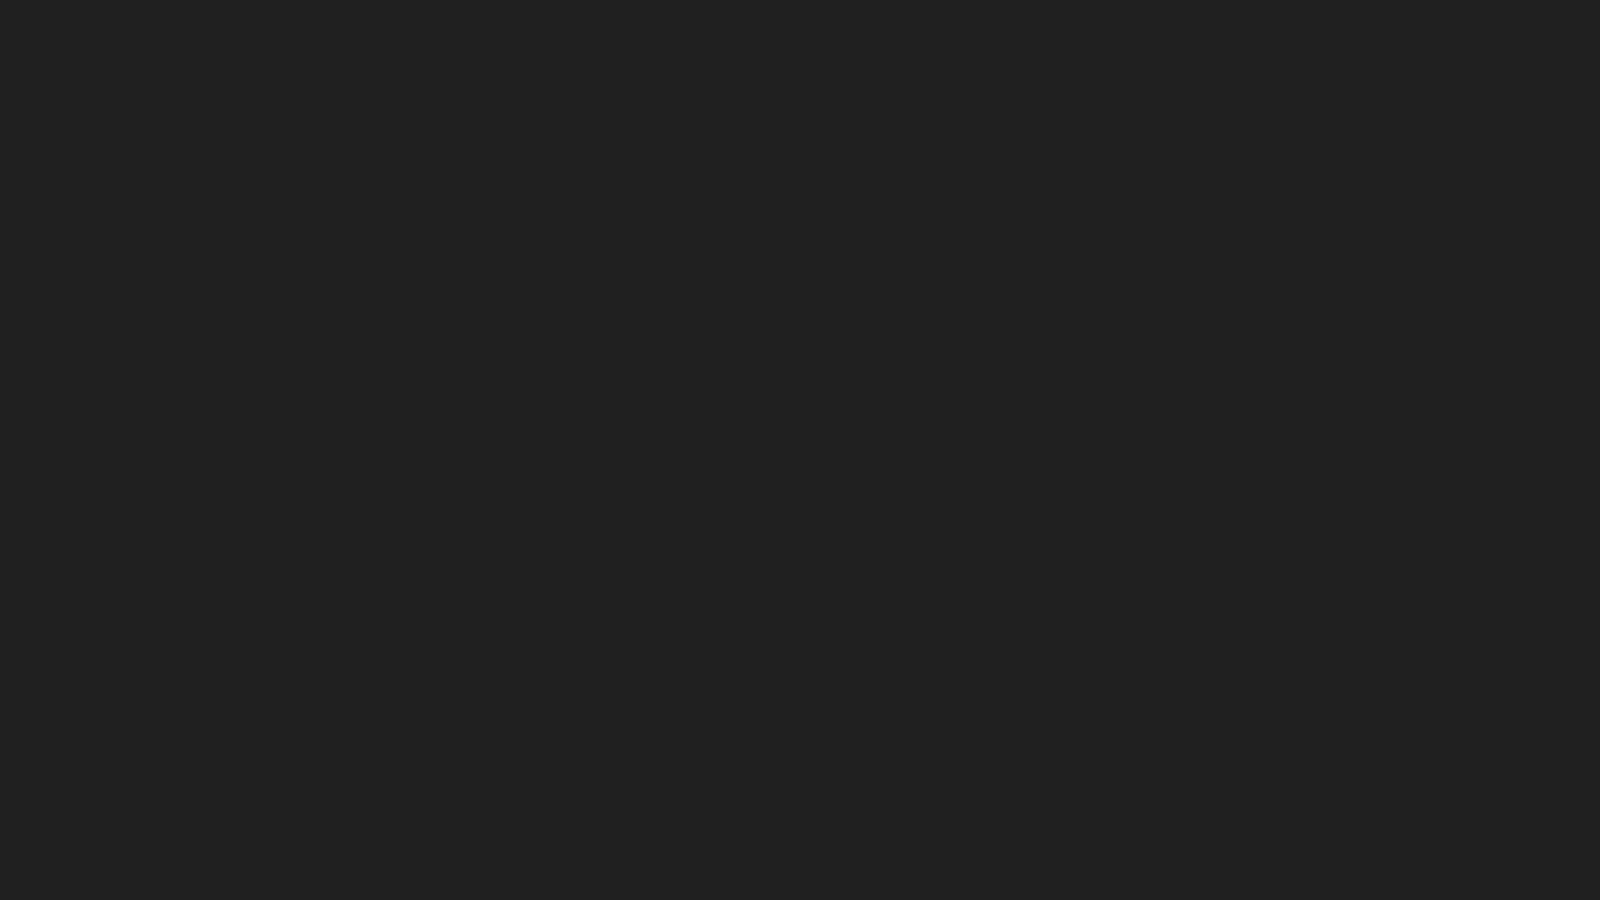
\includegraphics[width=\linewidth]{figure8.png}
  \caption{Implementation architecture placeholder: specification artifacts anchor scoped issue execution, AI-assisted generation produces repository-committed outputs, build validation and reflective audit checkpoints reconcile artifacts against architectural intent, and publication pipelines assemble final outputs from synchronized repository state.}
  \label{fig:figure8}
\end{figure}

\Cref{fig:figure8} anchors the implementation pipeline developed throughout this section and preserves deterministic figure references while the production diagram is being prepared.

\subsection{Specification-Driven Architecture}

Reflector treats specifications as synchronization anchors rather than as documentation afterthoughts. A specification in this sense is a structured artifact that describes what a system component, workflow, or publication process is expected to do, under what constraints it should operate, and what evidence would confirm that those expectations have been met. Specifications precede execution and survive it: they remain the reference point against which generated artifacts are evaluated at every subsequent checkpoint.

This role is analogous to the role of invariants in formally verified systems, but with a pragmatic orientation suited to mixed-initiative development \cite{Chandy1985DistributedSnapshots,Wiener1948Cybernetics}. A specification need not be machine-checkable in the formal verification sense; it must be inspectable by both humans and AI systems, sufficiently precise to guide scoped delegation, and stable enough to anchor reflective audit without requiring constant revision.

In practice, a specification-driven architecture organizes work across several artifact types:
\begin{itemize}
  \item \textbf{Architecture specifications} document system decomposition boundaries, layer responsibilities, and inter-component contracts, providing a stable reference for identifying boundary violations during audit.
  \item \textbf{Publication specifications} declare the semantic content structure, renderer targets, metadata requirements, and manifest formats that govern how outputs are assembled and distributed.
  \item \textbf{Workflow specifications} enumerate the phases of a recursive execution cycle---issue decomposition, delegation, generation, audit, synchronization---and specify the conditions that must hold before each transition.
  \item \textbf{Synchronization specifications} define checkpoint structures, evidence requirements, and continuation criteria, making the governance layer explicit rather than implicit in human judgment alone.
\end{itemize}

Together, these specification types form a recursive coordination infrastructure: each execution cycle begins by consulting the relevant specification, produces artifacts that can be checked against it, and terminates at a checkpoint where the specification remains available as the authoritative reference \cite{Beer1972BrainFirm}. This prevents the common failure mode in which recursive work gradually drifts away from its original conceptual commitments as artifacts and summaries accumulate.

\subsection{Repository-Centric Recursive Systems}

The repository is Reflector's primary memory substrate. Rather than relying on ephemeral conversation history or isolated agent state, Reflector persists recursive context in the repository: as issue threads that define execution boundaries, as committed artifacts that record generation outputs, as pull request deltas that expose local changes for review, and as workflow run logs that document execution history.

This design choice has significant consequences for recursive coherence. Repository-committed artifacts are versioned, addressable, and inspectable independently of the agent systems that produced them. Any participant---human or automated---can reconstruct the current state of a recursive workflow by reading the repository rather than by reconstructing conversational context from logs. This makes it possible to re-enter a recursive workflow at any checkpoint without losing the accumulated synchronization history \cite{Lamport1978TimeClocks}.

The repository-centric model maps directly onto widely available version control infrastructure:
\begin{itemize}
  \item \textbf{Issues} function as scoped execution boundaries with explicit acceptance criteria, constraining what a delegated task may change and what evidence it must produce.
  \item \textbf{Pull requests} function as synchronization checkpoints, making the diff between a prior stable state and a proposed new state inspectable before integration.
  \item \textbf{Commit history} functions as the recursive audit log, preserving the sequence of artifact transformations in a form that supports both retrospective review and incremental resumption.
  \item \textbf{Labels, milestones, and metadata} function as lightweight governance annotations, allowing teams to track which issues belong to which execution cycle and which checkpoints remain open.
\end{itemize}

This structure supports recursive depth without sacrificing traceability. As execution extends across many issues and cycles, the repository accumulates an inspectable record of decisions, artifacts, and synchronization events that makes architectural coherence verifiable rather than assumed \cite{Jimenez2024SWEBench,Yang2024SWEAgent}.

\subsection{Publication Architecture Patterns}

A publication-oriented system that applies Reflector principles organizes its output artifacts around a clean separation between semantic content and rendering concerns. Semantic content captures what is being communicated: the structure, argumentation, figures, and references of a document. Rendering concerns capture how that content should be presented: typography, layout, style, and target format. Conflating the two introduces unnecessary coupling that makes format migration, multi-target publishing, and incremental revision difficult to sustain recursively.

In practice, this separation is implemented through a layered architecture \cite{Parnas1972Modularization}:
\begin{itemize}
  \item \textbf{Content layer:} structured source files that carry semantic meaning without embedding presentation decisions. In a \LaTeX-based publication system, this corresponds to section files that contain argumentation and figure references but delegate all typographic decisions to a shared style layer.
  \item \textbf{Metadata layer:} centralized declarations of document identity, authorship, version, and status, maintained separately from content so that they can be updated without touching section files.
  \item \textbf{Style layer:} renderer packages or stylesheets that translate the semantic content into a target format. Swapping the style layer changes the visual output without altering the underlying content.
  \item \textbf{Manifest layer:} publication configuration files that declare which content, metadata, and style artifacts should be assembled for a given publication target, enabling deterministic and reproducible output.
\end{itemize}

This architecture supports recursive publication workflows because each layer can be audited and updated independently. A renderer upgrade does not require content changes; a metadata correction does not require rebuilding style assets. Synchronization checkpoints can therefore be scoped to individual layers, reducing the coordination surface for each publication cycle \cite{Vogels2009EventuallyConsistent}.

The manifest layer deserves particular attention because it makes publication intent explicit. Rather than relying on implicit toolchain conventions to determine what gets included in a publication artifact, a manifest file lists the precise inputs, their versions, and their target configurations. This enables deterministic reproduction of publication outputs from repository state alone, which is essential for both audit and archival requirements.

\subsection{Artifact Synchronization}

Recursive workflows accumulate many artifact types: source code, tests, documentation, figures, diagrams, generated summaries, specification files, and repository metadata. The synchronization challenge is not merely keeping each artifact individually current; it is maintaining consistency relationships across artifacts that reference, depend on, or constrain one another. A figure that depicts a workflow must remain consistent with the section that describes it; a specification that defines an interface must remain consistent with the implementation that realizes it.

Reflector addresses cross-artifact consistency through explicit synchronization checkpoints at which the artifact set is inspected as a whole rather than as isolated components. This is analogous to distributed snapshot protocols, which capture a consistent global state by coordinating across all system participants simultaneously rather than reading each participant independently \cite{Chandy1985DistributedSnapshots}. For recursive engineering workflows, the ``participants'' are the artifact types listed above, and the ``snapshot'' is the synchronized repository state at a given checkpoint.

Several artifact synchronization patterns emerge from this approach:
\begin{itemize}
  \item \textbf{Specification-artifact alignment:} generated code, tests, or documentation are checked against the specification that authorized their production, using the specification as the ground truth for scope conformance.
  \item \textbf{Cross-reference consistency:} figures, tables, and section references are validated to confirm that labeled artifacts exist, that their captions match their conceptual role, and that internal cross-references resolve correctly.
  \item \textbf{Metadata propagation:} version numbers, authorship fields, and status annotations are synchronized across all artifact types---source files, manifests, and repository metadata---so that the publication state remains coherent at the checkpoint level.
  \item \textbf{Dependency freshness:} generated artifacts that depend on upstream inputs are flagged for regeneration when upstream changes exceed a declared staleness threshold, preventing silent divergence between source and derived artifacts.
\end{itemize}

Together, these patterns make artifact synchronization a tractable recursive infrastructure rather than an ad hoc cleanup activity. When each checkpoint restores cross-artifact consistency, subsequent recursive cycles inherit a coherent foundation rather than accumulating hidden inconsistencies that compound over time \cite{Wiener1948Cybernetics,Beer1972BrainFirm}.

\subsection{Recursive Build and Validation Systems}

Publication and software artifacts require reproducible, automated build systems that validate outputs at every synchronization checkpoint. In recursive engineering workflows, a build system is not merely a compilation step; it is a recursive validation surface that confirms whether the current artifact set satisfies the consistency and quality requirements declared in the relevant specifications.

A Reflector-aligned build and validation system exhibits several properties:
\begin{itemize}
  \item \textbf{Reproducibility:} given a specific repository state, the build system produces identical outputs, making it possible to audit any historical checkpoint by re-running the build against the archived artifact set.
  \item \textbf{Staged validation:} validation runs in stages that correspond to the architectural layers described above, so that a failure in the metadata layer does not obscure unrelated failures in the content layer.
  \item \textbf{Artifact verification:} generated outputs are checked against declared expectations---figure file existence, bibliography completeness, manifest coverage---before being accepted as synchronization-ready artifacts.
  \item \textbf{Checkpoint integration:} the build system is coupled to the synchronization checkpoint workflow; a checkpoint is only considered complete when the build passes, establishing a direct link between checkpoint governance and artifact quality.
\end{itemize}

In practice, continuous integration infrastructure provides a natural home for recursive build validation \cite{Jimenez2024SWEBench}. Each pull request triggers a build that validates the proposed artifact set against the declared specifications; each merge into a stable branch represents an authorized synchronization event. This arrangement makes the CI system an automated participant in the reflective audit loop rather than a post hoc quality gate.

Recursive build systems also support publication reproducibility at the archival level. When a manuscript is submitted for publication, the artifact manifest and build configuration together provide the evidence needed to reproduce the submission from repository state. This capability is particularly important for recursive publication workflows, where the final artifact is the result of many iterative synchronization cycles rather than a single compilation pass.

\subsection{Human-AI Collaborative Tooling}

Reflector's implementation patterns are explicitly designed for collaborative operation between human engineers and AI systems. AI systems contribute high-throughput artifact generation---code, documentation, issue templates, figure scaffolds, and specification drafts---while human engineers contribute contextual judgment, acceptance decisions, and governance authority. The tooling layer must support this division clearly so that neither role is inadvertently undermined by the implementation.

Several tooling patterns support effective human-AI collaboration within a Reflector-aligned workflow \cite{Amershi2014InteractiveML,Shneiderman2020HCAI}:
\begin{itemize}
  \item \textbf{Specification-guided generation:} AI systems receive issue descriptions and specification context before execution, constraining their output surface to what the specification authorizes and making their generated artifacts directly auditable against the declared scope.
  \item \textbf{Inspectable artifact outputs:} all AI-generated artifacts are committed to the repository with attribution, making the generation provenance visible during audit rather than hidden in ephemeral session state.
  \item \textbf{Structured checkpoint handoff:} AI systems produce structured progress reports at delegation boundaries, summarizing what was changed, what evidence was generated, and what open questions remain for human review.
  \item \textbf{Bounded automation scope:} each delegated task has an explicit scope boundary that the AI system is expected to respect, preventing autonomous expansion into adjacent concerns that were not part of the authorized execution interval.
  \item \textbf{Reflective review loops:} human engineers review AI-generated artifacts against the originating specification before continuation, closing the audit loop and refreshing the authorization state before the next delegation cycle begins \cite{Sweller1988CognitiveLoad,Hutchins1995CognitionWild}.
\end{itemize}

The critical design principle is that humans remain the synchronization authorities. AI systems can accelerate scoped execution substantially, but the decisions that affect recursive trajectory---issue framing, acceptance criteria revision, checkpoint authorization, and scope expansion---remain governed by human judgment. This arrangement preserves the throughput advantages of AI assistance while maintaining the architectural coherence that recursive workflows require over extended timescales.

Practically, this means that the tooling layer should lower the cost of human review and oversight rather than attempting to eliminate it. Diff-oriented artifact presentation, specification-aligned change summaries, and auditable generation traces all reduce the cognitive overhead of checkpoint review, making effective human oversight compatible with the execution velocity that AI assistance enables \cite{Simon1957ModelsMan}.

\subsection{Transition Toward Future Systems}

The implementation patterns surveyed in this section---specification-driven architecture, repository-centric recursive memory, layered publication workflows, cross-artifact synchronization, recursive build validation, and human-AI collaborative tooling---together constitute a practically grounded realization of the Reflector architecture. Each pattern can be adopted incrementally and independently, allowing teams to introduce recursive synchronization infrastructure at the pace that their current workflows support.

Taken together, however, these patterns point toward a more general class of \textit{reflective infrastructure}: systems in which the engineering workflow itself is a first-class artifact that can be audited, versioned, and recursively improved using the same tools and principles that govern the software it produces. This generalization is significant because it suggests that the boundary between the engineering system and its product is not fixed. Repository workflows, specification systems, publication pipelines, and synchronization mechanisms can all be subject to the same reflective audit and bounded recursive improvement that Reflector applies to code and documentation artifacts.

Emerging directions for this class of systems include recursive developer experience platforms that adapt their own scaffolding based on synchronization history, publication operating systems that manage the full lifecycle from specification to archival distribution as a governed workflow, and synchronization-aware AI tooling that maintains explicit checkpoint state across long-horizon collaborative sessions. These directions share a common requirement: the infrastructure must remain inspectable, the synchronization events must remain explicit, and human governance authority must remain coupled to the moments that determine recursive trajectory.

The case studies examined in the following section (\Cref{sec:case-studies}) illustrate how these implementation patterns operate in concrete contexts, tracing specific recursive workflows from initial specification through artifact synchronization to publication-ready outputs. Those cases provide the empirical grounding for evaluating both the practical utility and the current limitations of the Reflector approach.

% \section{Case Studies}
\label{sec:case-studies}

Lorem ipsum dolor sit amet, consectetur adipiscing elit. Donec auctor nisi non sem gravida cursus. Vestibulum bibendum egestas leo, nec tristique tellus gravida quis.

A canonical reference to \Cref{fig:figure9} is included to stabilize the section's rendering skeleton.

\begin{figure}[H]
  \centering
  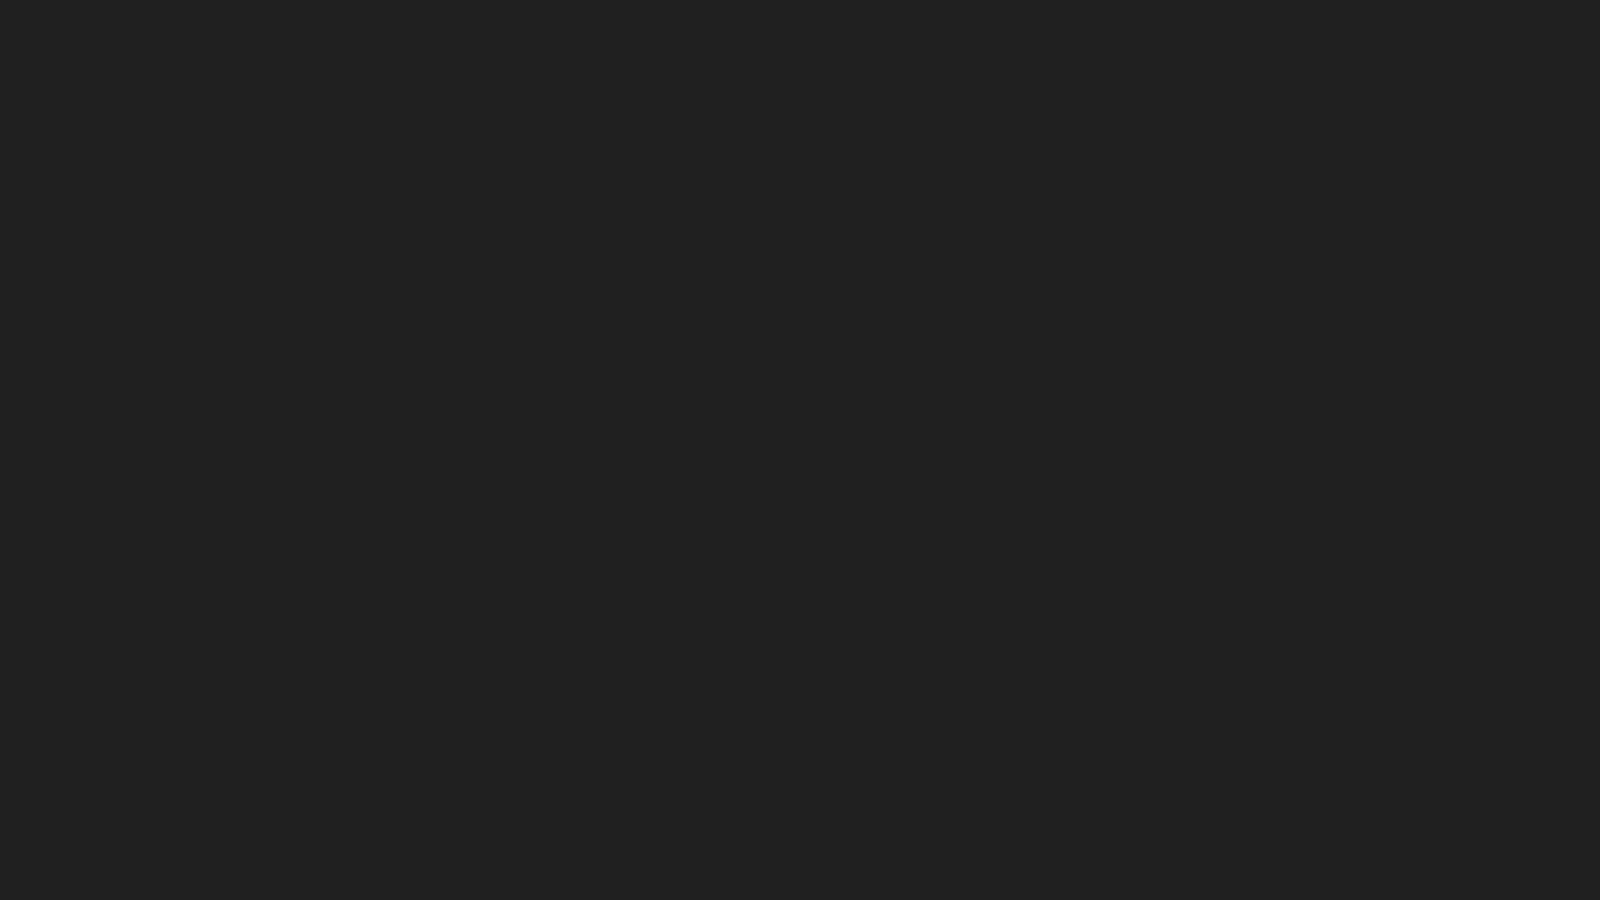
\includegraphics[width=\linewidth]{figure9.png}
  \caption{Placeholder case studies comparison figure.}
  \label{fig:figure9}
\end{figure}

\subsection{Comparative Placeholder}

Lorem ipsum dolor sit amet, consectetur adipiscing elit. Integer vulputate, dolor quis gravida iaculis, erat ligula feugiat sem, eget auctor mauris nisi nec mauris.


% ============================================================
% End Document
% ============================================================

\end{document}
